
\title{Типы и структуры данных}
\author[М. Кузнецов]{Максим Кузнецов}
\institute{ВШЭ, Москва}
\date{20 января 2016}

% Create title page.
\frame{\titlepage} 

%-------------------------------------------------------------------------------

\begin{frame}{Административное}
  
  {\bf Задачи}
  \begin{itemize}
    \item Листок 1 (анализ алгоритмов): 20.01 -- 27.01
    \item Листок 2 (структуры данных): 23.01 -- 03.02
  \end{itemize}

  В дальнейшем: листок рассылается после семинара, дедлайн -- следующий семинар.

  Задачи, слайды, вот это всё: \url{https://mkuznets.com/hse/2017-alg/}

  Примерный план лекций:
  \begin{itemize}
    \item L2: Структуры данных
    \item L3: Алгоритмы сортировки
    \item L4: Алгоритмы поиска
    \item L5: Графы
  \end{itemize}
  
\end{frame}

%-------------------------------------------------------------------------------

\begin{frame}{Абстрактные типы данных}
  
  {\bf АДТ} -- модель, представляющая объект данных через набор возможных принимаемых им значений, и операций над этим объектом и их свойств.

  {\bf Структура данных} -- конкретный способ реализации АДТ в компьютере.

  Выбор структуры данных во многом зависит от конструктивных ограничений и практической эффективности.

  \begin{itemize}
    \item $\mathds{Z}$ -- двоичная арифметика
    \item $\mathds{R}$ -- двоичные дроби (IEEE 754)%
      $$
      x = S \cdot M_n \cdot 2^{E_n},~~~ E_n \in \mathbb{Z},~ M_n \in [1, 2),~ S \in \{-1, 1\}
      $$ где $S$ --- знак, $M_n$ --- мантисса, а $E_n$ --- экспонента.
  \end{itemize}

  Компьютерная арифметика не полностью соответствует $\mathds{Z}$ и $\mathds{R}$, но хорошо работает на практике.
  
\end{frame}

%-------------------------------------------------------------------------------

\begin{frame}{Список (List)}
  
  {\bf Список} -- абстрактный тип данных соответствующий конечному упорядоченному набору (возможно, разнородных и повторяющихся) объектов.

  Операции:
  \begin{itemize}
    \item Доступ к элементам по порядковому номеру (индексу)
    \item Поиск элемента по значению
    \item Добавление элементов
    \item Удаление элементов
  \end{itemize}

  Структуры данных:
  \begin{itemize}
    \item Массив (Array)
      \begin{itemize}
        \item Статический
        \item Динамический
      \end{itemize}
    \item Связный список (Linked List)
  \end{itemize}


\end{frame}

%-------------------------------------------------------------------------------

\begin{frame}{Массив (Array)}
  
  {\bf Массив} -- {\em непрерывная} область памяти, содержащая $N$ смежных элементов фиксированного размера.

  Свойства:
  \begin{itemize}
    \item Компактность: элементы смежные, память не теряется
    \item {\em Поиск по индексу}: $O(1)$. Для элемента с индексом $n$:
      $$A_n = A_0 + S \cdot n$$
    \item {\em Добавление}: $O(n)$. При каждом добавлении придётся выделять новую память размера
      $S(N+1)$ и копировать все элементы.
    \item {\em Удаление}: $O(1)$ с концов (с потерей памяти). $O(n)$ из середины.
  \end{itemize}

\end{frame}

%-------------------------------------------------------------------------------

\begin{frame}{Связный список (Linked List)}
  
  Каждый элемент {\bf связного списка} содержит некоторое значение и адрес(а):
  \begin{itemize}
    \item следующего элемента (односвязный, singly-linked)
    \item предыдущего и следующего (двусвязный, doubly-linked)
  \end{itemize}


  Свойства:
  \begin{itemize}
    \item Издержки по памяти: $O(n)$
    \item {\em Поиск по индексу}: $O(n)$. Для элемента с индексом $k$ надо сделать $k$ <<прыжков>> по указателям.
    \item {\em Поиск по значению}: $O(n)$
    \item {\em Добавление/удаление}: $O(1)$ в начало, конец, или при уже известной позиции. Иначе $O(n)$.
  \end{itemize}

\end{frame}

%-------------------------------------------------------------------------------


\begin{frame}{Динамический массив (Dynamic Array)}
  
  {\bf Динамический массив} оптимизирует добавление и удаление элементов, сохраняя быстрый доступ по индексу.

  Простейший пример:%
  \begin{itemize}
    \item Оптимизирует только операции {\em на конце} массива. Вставка и удаление из середины по-прежнему $O(n)$
    \item Будем различать {\em ёмкость} (capacity) массива (размер выделеной памяти) от памяти, которую занимают элементы массива (logical size).
    \item Пусть размер массива удваивается когда не остаётся места для добавления новых элементов.
  \end{itemize}

\end{frame}

%-------------------------------------------------------------------------------

\begin{frame}{Динамический массив (Dynamic Array)}
  
\begin{figure}
  \centering
  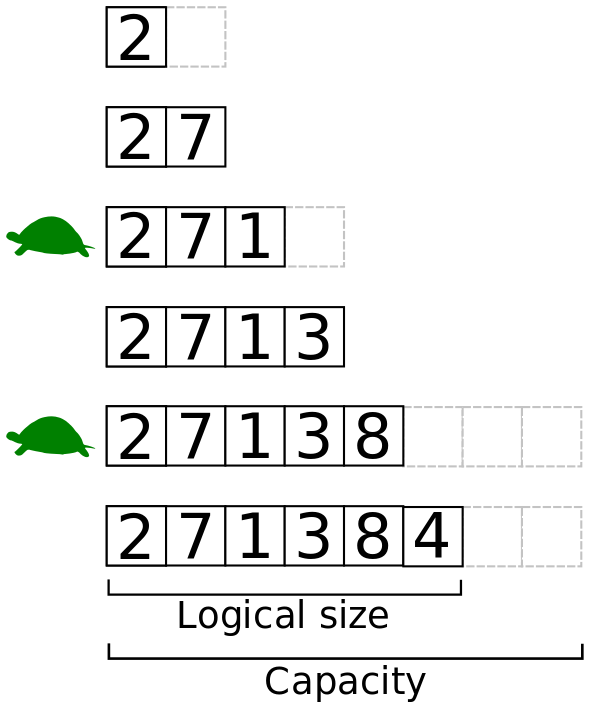
\includegraphics[width=7cm]{darray.png}
\end{figure}

\end{frame}

%-------------------------------------------------------------------------------

\begin{frame}{Динамический массив (Dynamic Array)}
  
Добавили $n$ элементов: $\log_2{n}$ <<удваиваний>>, $n/2$ элементов скопированы один раз, $n/4$ -- два раза, и так далее:
  $$
  M = \sum_{i=1}^{\log_2{N}} i \cdot n/2^i
    = n \sum_{i=1}^{\log_2{N}} i/2^i \leqslant
    = n \sum_{i=1}^{\infty} i/2^i < 2n ~~\sim~~O(n)
  $$
т.е. {\em амортизированная} стоимость одного добавления -- $O(1)$, хоть и некоторые из них будут медленнее.

Та же стратегия работает при удалении элементов с конца.

\end{frame}

%-------------------------------------------------------------------------------

\begin{frame}{\texttt{list} в Python}

\texttt{list} в Python реализован как описаный выше динамический массив:

\begin{table}
    \begin{tabular}{l|l}
    \hline
    Operation      & Amortized Worst Case \\ \hline
    \texttt{A.append(x)}    & O(1)                 \\ \hline
    \texttt{A.insert(x, k)} & O(n)                 \\ \hline
    \texttt{A[k]}           & O(1)                 \\ \hline
    \texttt{A[k] = x}       & O(1)                 \\ \hline
    \texttt{del A[k]}       & O(n)                 \\ \hline
    \texttt{A.index(x)}     & O(n)                 \\ \hline
    \texttt{min(A), max(A)} & O(n)                 \\ \hline
    \end{tabular}
\end{table}

\url{https://wiki.python.org/moin/TimeComplexity}

\end{frame}

%-------------------------------------------------------------------------------

\begin{frame}{Бинарный поиск (Binary Search)}

... он же двоичный поиск, бисекция, etc.

В отсортированном массиве можно искать быстрее:

\begin{figure}
  \centering
  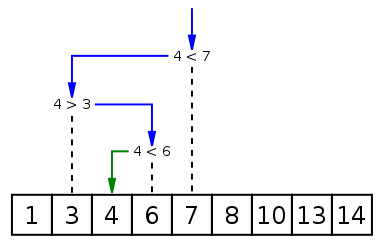
\includegraphics[width=8cm]{binarysearch.png}
\end{figure}

Сложность: $O(\log n)$ (доказать!)

\end{frame}

%-------------------------------------------------------------------------------

\begin{frame}[fragile]{Бинарный поиск}

Реализация на Python:
\begin{verbatim}
def binary_search(arr, value):
    low = 0
    high = len(arr)-1
    while low <= high: 
        mid = (low + high) // 2
        if arr[mid] > value: high = mid-1
        elif arr[mid] < value: low = mid+1
        else: return mid
    return -1
\end{verbatim}

\end{frame}

%-------------------------------------------------------------------------------

\begin{frame}[fragile]{Бинарный поиск}

Стандартный модуль \texttt{bisect} реализует бинарный поиск:
\begin{verbatim}
>>> from random import randint
>>> import bisect
>>> 
>>> arr = sorted([randint(10, 100) for i in range(10)])
>>> arr
[23, 37, 45, 48, 65, 69, 77, 85, 88, 93]
>>> bisect.bisect_left(arr, 77)
6
\end{verbatim}

\end{frame}

%-------------------------------------------------------------------------------

\begin{frame}[fragile]{Добавление + поиск}

Хочется добавлять элементы в структуру данных, а потом эффективно искать по ним:

\begin{itemize}
  \item Массив: быстрый поиск, медленное добавление
  \item Связный список: медленный поиск, быстрое добавление [как только нашли позицию]
\end{itemize}

Изобразим все варианты поиска элементов в массиве

\texttt{[1, 2, 3, 4, 5, 6, 7, 8, 9, 10, 11, 12, 13, 14, 15]}

\begin{figure}
  \centering
  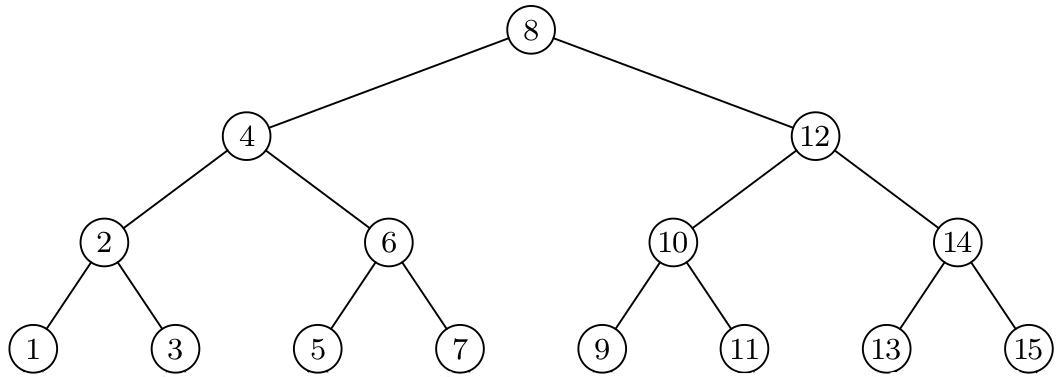
\includegraphics[width=10cm]{btree.png}
\end{figure}

\end{frame}

%-------------------------------------------------------------------------------


\begin{frame}[fragile]{Дерево (Tree)}

{\bf Дерево} --  связный граф без циклов.

\begin{itemize}
  \item Состоит из {\em узлов} (вершин, nodes), содержащих значение и $n$ ссылок на другие узлы -- {\em потомки} (children).
  \item {\em Корень} (root) -- узел, на который не ссылаются другие узлы. {\em Лист} (leave) -- узел, который не ссылается на другие узлы. Остальные узлы называются {\em внутренними} (inner). {\em Высота} -- максимальное расстояние от корня до листьев.
  \item {\em Поддерево} (subtree) -- любая некорневая вершина вместе с её потомками.
\end{itemize}

\begin{verbatim}
class TreeNode(object):
    def __init__(self, x, left=None, right=None):
        self.val = x
        self.left = left
        self.right = right

TreeNode(8, TreeNode(5), TreeNode(10))
\end{verbatim}


\end{frame}

%-------------------------------------------------------------------------------

\begin{frame}[fragile]{Бинарное дерево поиска (Binary Search Tree)}

{\bf Свойства}:

\begin{itemize}
  \item Каждый узел имеет два поддерева
  \item Уникальные значения в узлах
  \item Значение каждого узла больше всех значений в левом и меньше всех значений в правом поддереве
\end{itemize}

\begin{figure}
  \centering
  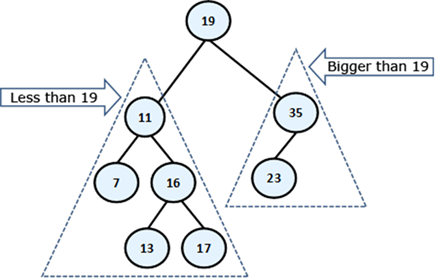
\includegraphics[width=5cm]{subtrees.png}
\end{figure}

\begin{itemize}
  \item Интуитивно: время поиска, добавления и удаления элементов {\bf пропорционально высоте дерева} (позже докажем сторого)
\end{itemize}

\end{frame}

%-------------------------------------------------------------------------------

\begin{frame}[fragile]{Бинарное дерево поиска (Binary Search Tree)}


\begin{itemize}
  \item Высота может варьироваться от $O(\log n)$ в {\em сбалансированном} (balanced) дереве, до $O(n)$ в вырожденном случае.
  \item Визуализация добавления элементов: \url{https://www.cs.usfca.edu/~galles/visualization/BST.html}
\end{itemize}

\begin{figure}
  \centering
  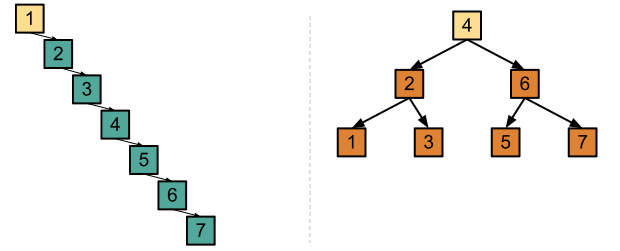
\includegraphics[width=8cm]{balance.png}
\end{figure}

\begin{itemize}
  \item Существуют {\em самобалансирующиеся} бинарные деревья где все операции требуют $O(\log n)$
  \item Дополнительная память на указатели: $O(n)$
\end{itemize}

\end{frame}

%-------------------------------------------------------------------------------
